%%%%%%%%%%%%%%%%%%%%%%%%%%%%%%%%%%%%%%%%%%%%%%%%%%%%%%%%%%%%%%%%%%%%%%%%
% Preamble
%%%%%%%%%%%%%%%%%%%%%%%%%%%%%%%%%%%%%%%%%%%%%%%%%%%%%%%%%%%%%%%%%%%%%%%%
\documentclass[11pt]{article}
%
% Packages and other includes
% Pagination
\usepackage[letterpaper, margin=1in]{geometry}
\usepackage{emptypage}
\usepackage{ulem}
\usepackage{xcolor}
\usepackage{mhchem}
%
% Fonts
\usepackage[T1]{fontenc} % best for Western European languages
\usepackage{lmodern} % Latin Modern instead of CM
\usepackage{textcomp} % required to get special symbols
%
% Math
\usepackage{amsmath, amssymb}
\usepackage{braket}
%
% Graphics, floats, tables
\usepackage{graphicx, color, float, array}
%
% Hyperlinks
\usepackage{hyperref}
%
%
% Definitions and settings
% Paragraph indent and spacing
\setlength{\parskip}{0.4\baselineskip}
\setlength{\parindent}{0in}
%
%
% Title, authors, date
\title{\textbf{Worksheet 8}}
\date{\vspace{-2em}March 4th, 2022}
%
%
%%%%%%%%%%%%%%%%%%%%%%%%%%%%%%%%%%%%%%%%%%%%%%%%%%%%%%%%%%%%%%%%%%%%%%%%
% Main document
%%%%%%%%%%%%%%%%%%%%%%%%%%%%%%%%%%%%%%%%%%%%%%%%%%%%%%%%%%%%%%%%%%%%%%%%
%

\begin{document}

\maketitle

Collaborations are encouraged and students must report all collaborators
on each assignment. All external sources (websites, books) must be
cited. An \textit{extra credit} (\textit{EC}) problem will be available per
assignment. Please submit a completed homework on-time to receive \textit{EC}
and no partial \textit{EC} (all parts must be correct) will be given out.
Additional problems are listed at the end of each assignment. This week's
assignment is due \textit{Tuesday, March 8th at 2:00pm.}

1. (5 pts) \textbf{Phase Diagram} The phase diagram for carbon is shown in Fig. \ref{fig:carb}.
Answer the following questions:

(a) At 3000K, what is the minimum pressure needed before graphite changes into
diamond? At the phase change, determine the degrees of freedom using Gibbs phase rule.

(b) What is the triple point temperature $T_p$ for carbon? At the triple point,
determine the degrees of freedom using Gibbs phase rule.

(c) Based on the phase diagram, are diamonds stable under normal conditions e.g.
1 atm and room temperature? If not, why are people able to wear diamonds without
keeping them under high pressure?

\begin{figure}[hbpt]
  \centering
  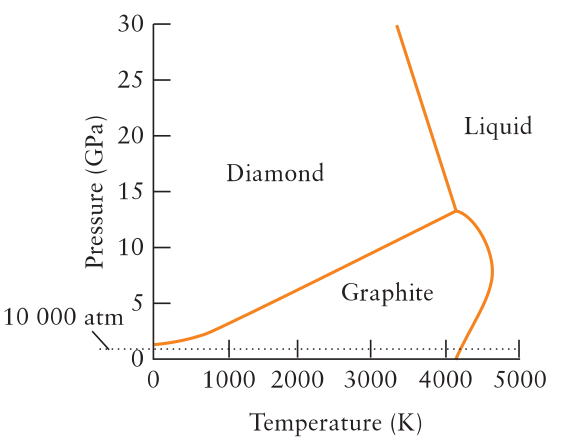
\includegraphics[scale=0.4]{carbon.png}
  \caption{Phase diagram for carbon}
  \label{fig:carb}
\end{figure}

\pagebreak

2. (3 pts) \textbf{Vapor Pressure} Explain how the vapor pressure of a liquid is affected
by each of the following changes in conditions:

(a) an increase in temperature

(b) a decrease in surface area of the liquid

(c) an increase in the surface tension

\vspace{2in}

%3. (5 pts) \textbf{Vapor Pressure} The vapor pressure of phosphoryl chloride
%difluoride (OPClF$_2$) has been measured as a function of temperature:
%\begin{table}[hbpt]
%  \centering
%  \begin{tabular}{cc}
%    Temperature (K) & Vapor pressure (Torr) \\
%    \hline
%    190 & 3.2 \\
%    228 & 68 \\
%    250 & 240. \\
%    273 & 672
%  \end{tabular}
%  \caption{Reported vapor pressure at various temperatures.}
%\end{table}
%
%(a) Plot $\ln P$ against $1/T$.
%
%(b) From the plot, determine the standard enthalpy of vaporization $\Delta H_\text{vap}$,
%and standard entropy of vaporization $\Delta S_\text{vap}$.
%
%(c) If the pressure of a sample of OPClF$_2$ is reduced to 15 Torr, at what
%temperature will the sample boil?
%
%\pagebreak

3. (4 pts) \textbf{Clausius--Clapeyron Equation} The Clausius--Clapeyron equation
relates the vapor pressure and temperature of the system given by
\begin{equation}
  P_f = P_i e^{-\frac{\Delta H^\circ_\text{vap}}{R}(\frac{1}{T_2}-\frac{1}{T_1})}
\end{equation}
where $P$ is the vapor pressure, $T$ is the temperature, and $\Delta H^\circ_\text{vap}$
is the enthalpy of vaporization. Report results to 3 significant figures.

(a) At standard atmospheric pressure, the vapor pressure of water at 80$^\circ$C is
355.26 Torr. Determine the $\Delta H^\circ_\text{vap}$ for water. \textit{Hint:} What is the
vapor pressure of water at $100^\circ$C?

(b) Using $\Delta H^\circ_\text{vap}$ in part (a), determine the amount of energy
needed to heat 1 L of water from $10^\circ$C to $120^\circ$C? Heat capcities of liquid
water and water vapor are 4.184 J/(g $^\circ$C) and 1.996 J/(g $^\circ$C), respectively.

\pagebreak

4. (7 pts) \textbf{Real Gases} The Van der Waals equation extends the ideal gas equation to
include the effects of interaction between molecules of a gas given by
\begin{equation}
  (P+\frac{a}{v^2})(v - b) = RT
  \label{eqn:van_der}
\end{equation}
where $P$ is the pressure, $v$ is the molar volume, $T$ is the temperature, $a$ and $b$
are constants accounting for the non-ideality of the gas. Iron pyrite, FeS$_2$, is the
form in which much of the sulfur exists in coal. In the combustion of coal, oxygen reacts
with FeS$_2$ to produce iron(III) oxide and sulfur dioxide, which is a major source of air
pollution and contributes to acid rain. The van der Waals parameters for SO$_2$ are
$a = 6.865$ L$^2$ atm mol$^{-2}$ and $b = 0.0568$ L mol$^{-1}$.

(a) Write a balanced equation for the burning of FeS$_2$ in air to produce iron(III)
oxide and sulfur dioxide. Include states.

(b) For SO$_2$ confined in a 1.00 L vessel at 32$^\circ$C, calculate the pressure of the gas
by using the ideal gas law and the van der Waals equation for 0.100 mol to 1.100 mol SO$_2$ at
0.200 mol increments.

(c) Calculate the percentage deviation of the ideal value from the van der Waals equation at
each point in part (b).

(d) If we consider gases to be ideal when the observed pressure differs by no more than $5\%$
from the ideal value, at what pressure does SO$_2$ become a ``real'' gas?

\pagebreak

%6. (2 pts) \textbf{Van der Waals Constants $a$ and $b$} In eqn. \ref{eqn:van_der}, the constants
%$a$ and $b$ may be viewed as corrections to the ideal gas. $a$ accounts for the strength
%of attractions between its component molecules whereas $b$ considers the finite volume
%that the molecule occupies.


5. (4 pts) \textbf{Phase Changes} \textit{Extra Credit:} Let's interpret phase changes in terms
of the thermodynamic functions. Consider the plot of the temperature dependence of the molar
Gibbs free energy $G_m$ of the three phases of a substance in Fig. \ref{fig:gibbs_phase}.

(a) Indicate on the plot what is most favored phase for each section? At each intersection,
what is this indicating?

(b) Explain in terms of molecular behavior why the $G_m$ of each phase decreases with temperature.

(c) Explain in terms of molecular behavior why the $G_m$ of the vapor phase decreases more rapidly
with temperature than that of the solid or liquid phase.

\begin{figure}[hbpt]
  \centering
  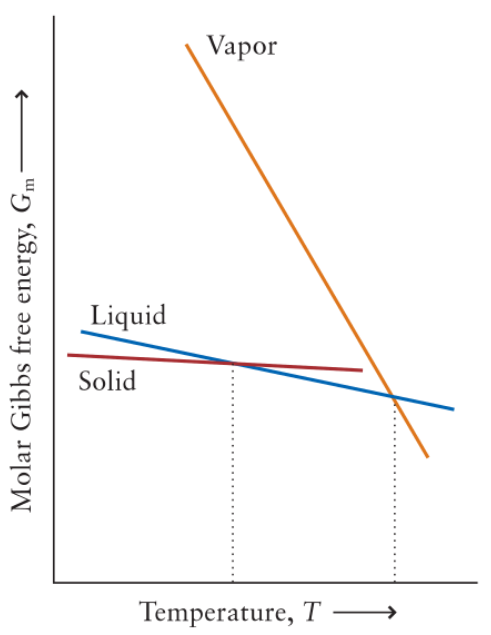
\includegraphics[scale=0.3]{gibbs_phases.png}
  \caption{Gibbs free energy for three phases of a substance at a given
    pressure.}
  \label{fig:gibbs_phase}
\end{figure}


\pagebreak

6. (10 pts) \textbf{Noncovalent Interactions} \textit{Extra Extra Credit:}
In lecture, Prof. Furche mentioned your TA Brian's Ph.D. work on noncovalent interactions (NIs).
These include electrostatic, induction, and dispersion. The textbook description of
dispersion is that these are instantaneous dipole moments and relatively ``weak'' compared to
covalent bonds. However, this is not necessarily the correct interpretation. Attached is your TA Brian's
\href{https://doi.org/10.1021/acs.jctc.9b01176}{\textit{landmark} publication}.

(a) Provide examples where NIs are important. Cite your sources.

(b) According to the paper, summarize the main results and conclusions.

(c) Given Fig. \ref{fig:nis} taken from the paper, how should we physically interpret NIs?
\begin{figure}[hbpt]
  \centering
  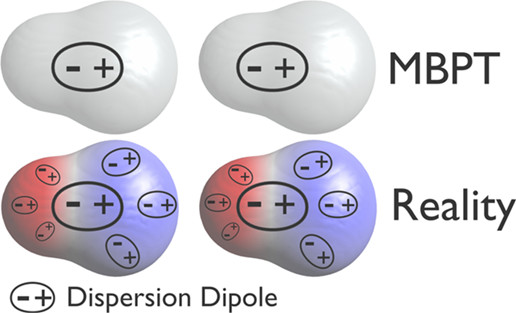
\includegraphics[scale=1.5]{dispersion.jpeg}
  \caption{Illustration of dispersion interactions.}
  \label{fig:nis}
\end{figure}

Partial credit may be given out. \textit{Hint:} Attend Prof. Furche and Brian's office hours.
\textbf{Due: March 14, 2022, at 10:30am}

\vfill
\textbf{Optional Additional Problems:} Ch. 11 - odd problems $35 - 45$, $53 - 89$

\end{document}
